\documentclass[11pt,letterpaper]{article}
\usepackage[utf8]{inputenc}
\usepackage{caption} % for table captions
\usepackage{amsmath} % for multi-line equations and piecewises
\usepackage{graphicx}
%\usepackage{textcomp}
\usepackage{xspace}
\usepackage{verbatim} % for block comments
%\usepackage{subfig} % for subfigures
\usepackage{enumitem} % for a) b) c) lists
\newcommand{\Cyclus}{\textsc{Cyclus}\xspace}%
\newcommand{\Cycamore}{\textsc{Cycamore}\xspace}%
\usepackage{tabularx}
\usepackage{color}
\definecolor{bg}{rgb}{0.95,0.95,0.95}
\newcolumntype{b}{X}
\newcolumntype{f}{>{\hsize=.15\hsize}X}
\newcolumntype{s}{>{\hsize=.5\hsize}X}
\newcolumntype{m}{>{\hsize=.75\hsize}X}
\newcolumntype{r}{>{\hsize=1.1\hsize}X}
\usepackage{titling}
\usepackage[hang,flushmargin]{footmisc}
\renewcommand*\footnoterule{}
\usepackage[newfloat]{minted}
\newenvironment{code}{\captionsetup{type=listing}}{}
\SetupFloatingEnvironment{listing}{name=Code}
\newcolumntype{P}[1]{>{\centering\arraybackslash}p{#1}}

\usepackage{tikz}


\usetikzlibrary{shapes.geometric,arrows}
\tikzstyle{process} = [rectangle, rounded corners, minimum width=1cm, minimum height=1cm,text centered, draw=black, fill=blue!30]
\tikzstyle{arrow} = [thick,->,>=stealth]


\graphicspath{{images/}}
 
\title{Numerical Experiments for Verifying Demand Driven Deployment Algorithms \\ \vspace{0.5em} \textbf{\large{Non-Optimizing Method}}}
\author{Jin Whan Bae, Gwendolyn Chee, Kathryn Huff}


\begin{document}
	\maketitle
	\hrule

\section{Introduction}
For many fuel cycle simulations, it is currently up to the user to define
a deploy scheme, or facility parameters, to make sure that there's no gap
in the supply chain. Or, the same goal is achieved by setting the
\texttt{facility} capacity to infinity, which does not reflect real-world
conditions. 

The Demand-Driven Cycamore Archetype project (NEUP-FY16-10512) aims to develop \Cycamore demand-driven deployment capabilities.
The developed algorithm, in the form of \Cyclus \texttt{Institution}
agent, deploys \texttt{Facilities} to meet the front-end and back-end demands of the 
fuel cycle.

This report describes numerical tests for non-optimizing, deterministic-optimizing and stochastic-optimizing prediction algorithms.

These prediction models are being developed by the University of South Carolina. 
In this report, we discuss numerical experiments for testing the non-optimizing, 
deterministic optimizing and stochastic optimizing methods. The numerical 
experiments will be designed for both the once through nuclear fuel 
cycle and advanced fuel cycles. 

\section{Method}
This report lists necessary capabilities of the new \Cyclus \texttt{institute}
for demand-driven deployment of fuel cycle facilities. 
Then the report lists tests to check correct implementation of the capabilities,
with a sample fuel cycle with well-defined facility parameters.


\section{Configuration}
The user defines prototypes to be deployed for fuel facilities,
and reactor deployment scheme.  The reactor deployment causes the demand of fuel
which triggers fuel facility deployment. The detailed input file XML input schema
is shown in Appendix A. 

\section{Algorithm Flow}

The algorithm, upon entering, creates a supply chain with the fuel facilities and
the reactor. Then, at every timestep it calculates the expected demand from each fuel cycle
facility and makes decisions to deploy or decommission. As a reference, the time step
execution for \Cyclus is illustrated in figure \ref{diag:time}.

\begin{figure}[H]
\centering
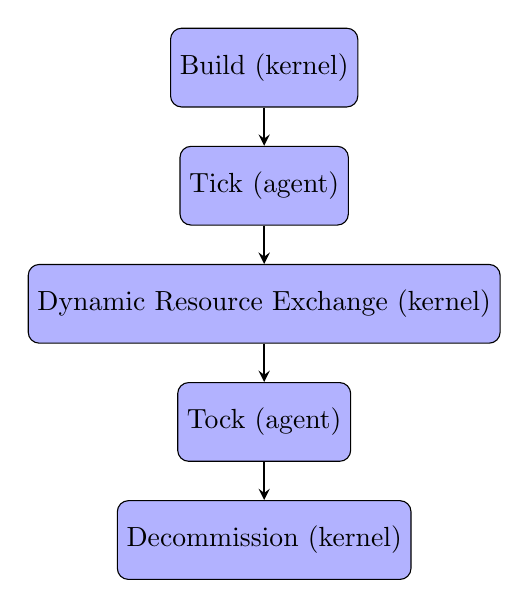
\begin{tikzpicture}[node distance=1.5cm]
\node (Build) [process] {Build (kernel)};
\node (Tick) [process, below of=Build] {Tick (agent)};
\node (DRE) [process, below of=Tick]{Dynamic Resource Exchange (kernel) };
\node (Tock) [process, below of=DRE]{Tock (agent)};
\node (Decom) [process, below of=Tock] {Decommission (kernel)};

\draw [arrow] (Build) -- (Tick); 
\draw [arrow] (Tick) -- (DRE);
\draw [arrow] (DRE) -- (Tock);
\draw [arrow] (Tock) -- (Decom);
\end{tikzpicture}
\caption{Each timestep in \Cyclus follows the five steps in order. Processes labeled
         kernel are executed by the \Cyclus framework, whereas processes labeled agent
         are executed by individual agents. What happens in the `Tick' and `Tock' is
         thus unique to each archetype.}
\label{diag:time}
\end{figure}

\subsection{Upon Entering (\texttt{Enternotify})}

The algorithm creates a supply chain with the fuel facilities,
then calculates the demand for each facility for a unit quantity of fuel
(example in figure \ref{diag:dem}). It also orders to build fuel cycle
facilities for the reactors at timestep 1.

\begin{figure}[H]
\centering
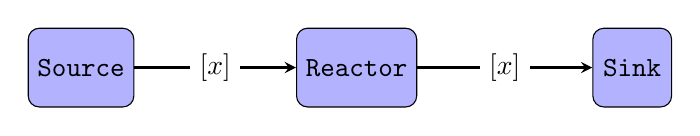
\begin{tikzpicture}[node distance=3.5cm]
\node (source) [process] {\texttt{Source}};
\node (reactor) [process, right of=source]{\texttt{Reactor}};
\node (sink) [process, right of=reactor]{\texttt{Sink}};

\draw [arrow] (source) -- (reactor) node[midway,fill=white] {$[x]$}; 
\draw [arrow] (reactor) -- (sink) node[midway,fill=white] {$[x]$}; 
\end{tikzpicture}
\caption{Simple demand flow of materials. The values in the bracket are demands calculated
         by the algorithm. The \texttt{Reactor} demands $x$ amount of fuel,
         which translates into demands of $x$ from  \texttt{Sink}.}
\label{diag:dem}
\end{figure}

\subsection{Tick}
The algorithm calculates the fuel demand
from the fleet of reactors at one timestep ahead, and the corresponding demand for fuel facilities.
The current capacity of each fuel cycle facility is also calculated. If the capacity
is smaller than the demand, the algorithm orders to build more facilities to meet the demand,
so that the fuel demand is met for the next timestep.

\section{Simulation parameter for Test Scenarios}
Simple parameters are given to fuel cycle facilities for the numerical testing of 
the algorithm.  Only \texttt{source} and \texttt{reactor} facilities are used in the test scenarios. 

Table \ref{tab:testscenario} provides basic parameters for each test scenario. Table \ref{tab:reactor} provides the parameters for the \texttt{source}, \texttt{reactors} and \texttt{sink} in the test scenarios.

\begin{table}[H]
	\centering
	\caption {Basic Test Parameters}
	\label{tab:testscenario}
	\begin{tabular}{|l|l|l|}
		\hline
		\textbf{Test Scenario Parameters} & \textbf{Value} & \textbf{Units} \\
		\hline
		Duration & 15 & timesteps \\
		Timestep & 1 & month \\
		Start Month & 1 & month \\
		Start Year & 2000 & year \\
		\hline
	\end{tabular}
\end{table}

\begin{table}[H]
	\centering
    \caption {Source, Reactor and Sink Parameters}
	\label{tab:reactor}
	\begin{tabular}{|l|l|l|}
\hline
\textbf{Source Parameters} & \textbf{Value} & \textbf{Units} \\
\hline
Throughput & 1 & kg \\
Output Commodity & fuel & kg\\
\hline
\textbf{Reactor Parameters} & \textbf{Value} & \textbf{Units} \\
\hline
Cycle Time & 1 & timesteps \\
Refuel Time & 0 & timesteps \\
Lifetime & 1 & timesteps \\
Power Capacity & 1& MWe \\
Assembly Size & 1 & kg \\
\# assemblies per core & 1 & \\
\# assemblies per batch & 1 & \\
Input Commodity & fuel & kg\\
Output Commodity & power & MW\\
\hline
\textbf{Sink Parameters} & \textbf{Value} & \textbf{Units} \\
Throughput & 1 & kg \\
Input Commodity & spent uox & kg\\
\hline
	\end{tabular}
\end{table}

\pagebreak

\section{Numerical Tests for the Non-optimizing prediction method}
The non-optimizing prediction method is tested by comparing its output for various scenarios against their analytical solutions . In this section, the tests that must be met is described based on the parameters defined in table \ref{tab:testscenario} and \ref{tab:reactor} and analytical solution of a defined simple scenario. Unit test examples are included in Appendix B.

The tests are split into test A types and test B types. Test A refers to the test scenarios where facilities are expected to be deployed. Test B refers to the test scenarios where facilities are expected to be decommissioned. 

The prediction algorithm for the non-optimizing method has three user-defined input parameters. The aim of the various test scenarios are to check if the non-optimizing method archetype will deploy or decommission facilities correctly when there is a variation in the combination of the three input parameters.  The input parameters are: 
\begin{enumerate}
	\item Initial demand value  
	\item Number of initial facilities (initial supply)
	\item Growth rate of initial demand
\end{enumerate}

The growth in demand is governed by the Equation \ref{eq:growth}. 

\begin{align}
\label{eq:growth}
D_f(timestep) &= D_i(1+g)^{(\frac{timestep}{12})}
\end{align}
Where $D_f$ is demand of resource at specific time step, $D_i$ is initial demand and g is growth rate. 

\texttt{Source} and \texttt{reactor} facilities are used in the test scenarios. Test scenarios A1 to A4 and B1 to B2 only have a \texttt{source} facility and test scenarios A5 to A7 have both \texttt{source} and \texttt{reactor} facilities. For each test scenario, there is one table that states the test scenario's input parameters and another table that states the exact analytical solution. The analytical solution table does not include deployment of the initial facility that is stated in the first table.

Additionally, we created base tests for each A-type test scenario that passes when the supply meets the demand within a given facility number tolerance. In other words, when the supply exceeds the demand by the specified tolerance quantity, the test still passes. For this report, the tolerance is set to one facility. For example in test A-1, the expected total number facilities deployed is 1, and since the facility over-prediction tolerance is 1, the acceptable range of total number of facilities $(x)$ deployed in the entire test scenario is $1<x<2$. If the total number of facilities deployed is within this range, the base case test will pass.  

\subsection{Test A-1}
In test A-1, only a \texttt{source} facility is present in the test scenario. Table \ref{tab:testa1} shows the input parameters of the source facility in the test scenario. Table \ref{tab:testa1ana} shows the expected analytical solution based on the test scenario. Table \ref{tab:testa1base} shows the accepted range of total number of facilities deployed over the test scenario which will pass the base test, which factors in the facility over-prediction tolerance of 1. 
\begin{table}[H]
	\centering
	\caption{Test A-1 Scenario Input Parameters }
	\label{tab:testa1}
	\begin{tabular}{|l|l|l|}
		\hline
		\textbf{Source Parameter} & \textbf{Value} & \textbf{Units} \\
		\hline
		Initial demand & 1 & kg \\
		Initial facilities & 0 & \#\\
		Growth Rate & 0 & \\
\hline
	\end{tabular}
\end{table}

\begin{table}[H]
	\centering
	\caption{Test A-1 Analytical Solution}
	\label{tab:testa1ana}
	\begin{tabular}{|l|l|}
		\hline
		\textbf{Time Step} & \textbf{\shortstack{No. of Source \\Facilities Deployed}}\\
		\hline
		1 & 1\\
		2 to 15& 0 \\
		\hline
	\end{tabular}
\end{table}

\begin{table}[H]
	\centering
	\caption{Test A-1 Base Test Acceptance}
	\label{tab:testa1base}
	\begin{tabular}{|P{6.5cm}|}
		\hline
		\textbf{\shortstack{Acceptable total No. of Source \\Facilities Deployed + tolerance}}\\
		\hline
		1 $<$ x $<$ 2 \\
		\hline
	\end{tabular}
\end{table}

\subsection{Test A-2}
In test A-2, only a \texttt{source} facility is present in the test scenario. Table \ref{tab:testa2} shows the input parameters of the source facility in the test scenario. Table \ref{tab:testa2ana} shows the expected analytical solution based on the test scenario.Table \ref{tab:testa2base} shows the accepted range of total number of facilities deployed over the test scenario which will pass the base test, which factors in the facility over-prediction tolerance of 1. 

\begin{table}[H]
	\centering
	\caption{Test A-2 Scenario Input Parameters }
	\label{tab:testa2}
	\begin{tabular}{|l|l|l|}
		\hline
		\textbf{Source Parameter} & \textbf{Value} & \textbf{Units} \\
		\hline
		Initial demand & 2 & kg \\
		Initial facilities & 1 & \#\\
		Growth Rate & 0 & \\
		\hline
	\end{tabular}
\end{table}

\begin{table}[H]
	\centering
	\caption{Test A-2 Analytical Solution}
	\label{tab:testa2ana}
	\begin{tabular}{|l|l|}
		\hline
		\textbf{Time Step} & \textbf{\shortstack{No. of Source \\Facilities Deployed}}\\
		\hline
		1 & 1\\
		2 to 15& 0 \\
		\hline
	\end{tabular}
\end{table}

\begin{table}[H]
	\centering
	\caption{Test A-2 Base Test Acceptance}
	\label{tab:testa2base}
	\begin{tabular}{|P{6.5cm}|}
		\hline
		\textbf{\shortstack{Acceptable total No. of Source \\Facilities Deployed + tolerance}}\\
		\hline
		2 $<$ x $<$ 3 \\
		\hline
	\end{tabular}
\end{table}

\subsection{Test A-3}
In test A-3, only a \texttt{source} facility is present in the test scenario. Table \ref{tab:testa3} shows the input parameters of the source facility in the test scenario. Table \ref{tab:testa3ana} shows the expected analytical solution based on the test scenario. Table \ref{tab:testa3base} shows the accepted range of total number of facilities deployed over the test scenario which will pass the base test, which factors in the facility over-prediction tolerance of 1. 

\begin{table}[H]
	\centering
	\caption{Test A-3 Scenario Input Parameters}
	\label{tab:testa3}
	\begin{tabular}{|l|l|l|}
		\hline
		\textbf{Source Parameter} & \textbf{Value} & \textbf{Units} \\
		\hline
		Initial demand & 1 & kg \\
		Initial facilities & 0 & \#\\
		Growth Rate & 1 &  \\
		\hline
	\end{tabular}
\end{table}

\begin{table}[H]
	\centering
	\caption{Test A-3 Analytical Solution}
	\label{tab:testa3ana}
	\begin{tabular}{|l|l|}
		\hline
		\textbf{Time Step} & \textbf{\shortstack{No. of Source \\Facilities Deployed}}\\
		\hline
		1 & 2\\
		2 to 12 & 0 \\
		13 & 1 \\
		14 to 15 & 0 \\
		\hline
	\end{tabular}
\end{table}

\begin{table}[H]
	\centering
	\caption{Test A-3 Base Test Acceptance}
	\label{tab:testa3base}
	\begin{tabular}{|P{6.5cm}|}
		\hline
		\textbf{\shortstack{Acceptable total No. of Source \\Facilities Deployed + tolerance}}\\
		\hline
		3 $<$ x $<$ 4 \\
		\hline
	\end{tabular}
\end{table}

\subsection{Test A-4}
In test A-4, only a \texttt{source} facility is present in the test scenario. Table \ref{tab:testa4} shows the input parameters of the source facility in the test scenario. Table \ref{tab:testa4ana} shows the expected analytical solution based on the test scenario. Table \ref{tab:testa4base} shows the accepted range of total number of facilities deployed over the test scenario which will pass the base test, which factors in the facility over-prediction tolerance of 1. 

\begin{table}[H]
	\centering
	\caption{Test A-4 Scenario Input Parameters }
	\label{tab:testa4}
	\begin{tabular}{|l|l|l|}
		\hline
		\textbf{Source Parameter} & \textbf{Value} & \textbf{Units} \\
		\hline
		Initial demand & 1 & kg \\
		Initial facilities & 1 & \#\\
		Growth Rate & 1 &  \\
		\hline
	\end{tabular}
\end{table}

\begin{table}[H]
	\centering
	\caption{Test A-4 Analytical Solution}
	\label{tab:testa4ana}
	\begin{tabular}{|l|l|}
		\hline
		\textbf{Time Step} & \textbf{\shortstack{No. of Source \\Facilities Deployed}}\\
		\hline
		1 & 1\\
		2 to 12 & 0 \\
		13 & 1 \\
		14 to 15 & 0 \\
		\hline
	\end{tabular}
\end{table}

\begin{table}[H]
	\centering
	\caption{Test A-4 Base Test Acceptance}
	\label{tab:testa4base}
	\begin{tabular}{|P{6.5cm}|}
		\hline
		\textbf{\shortstack{Acceptable total No. of Source \\Facilities Deployed + tolerance}}\\
		\hline
		3 $<$ x $<$ 4 \\
		\hline
	\end{tabular}
\end{table}

\subsection{Test A-5}
In test A-5, both a \texttt{source} and \texttt{reactor} facility is present in the test scenario. Table \ref{tab:testa5} shows the input parameters of the source facility in the test scenario. Table \ref{tab:testa5ana} shows the expected analytical solution based on the test scenario. Table \ref{tab:testa5base} shows the accepted range of total number of facilities deployed over the test scenario which will pass the base test, which factors in the facility over-prediction tolerance of 1. 

\begin{table}[H]
	\centering
	\caption{Test A-5 Scenario Input Parameters}
	\label{tab:testa5}
	\begin{tabular}{|l|l|l|}
		\hline
		\textbf{Source Parameter} & \textbf{Value} & \textbf{Units} \\
		\hline
		Initial demand & 1 & kg \\
		Initial facilities & 0 & \#\\
		Growth Rate & 0 &  \\
		\hline
		\textbf{Reactor Parameter} & \textbf{Value} & \textbf{Units} \\
		\hline
		Initial demand & 1 & MW \\
		Initial facilities & 0 & \#\\
		Growth Rate & 0 &  \\
		\hline
	\end{tabular}
\end{table}

\begin{table}[H]
	\centering
	\caption{Test A-5 Analytical Solution}
	\label{tab:testa5ana}
	\begin{tabular}{|l|l|l|}
		\hline
		\textbf{Time Step} & \textbf{\shortstack{No. of Source \\Facilities Deployed}} & \textbf{\shortstack{No. of Reactor \\Facilities Deployed}}\\
		\hline
		1 & 1 & 1\\
		2 to 15 & 0 & 0\\
		\hline
	\end{tabular}
\end{table}

\begin{table}[H]
	\centering
	\caption{Test A-5 Base Test Acceptance}
	\label{tab:testa5base}
	\begin{tabular}{|P{6.5cm}|P{6.5cm}|}
		\hline
		\textbf{\shortstack{Acceptable total No. of Source \\Facilities Deployed + tolerance}} &\textbf{\shortstack{Acceptable total No. of Reactor \\Facilities Deployed + tolerance}}\\
		\hline
		1 $<$ x $<$ 2 & 1 $<$ x $<$ 2\\
		\hline
	\end{tabular}
\end{table}

\subsection{Test A-6}
In test A-6, both a \texttt{source} and \texttt{reactor} facility is present in the test scenario. Table \ref{tab:testa6} shows the input parameters of the source facility in the test scenario. Table \ref{tab:testa6ana} shows the expected analytical solution based on the test scenario. Table \ref{tab:testa6base} shows the accepted range of total number of facilities deployed over the test scenario which will pass the base test, which factors in the facility over-prediction tolerance of 1. 

\begin{table}[H]
	\centering
	\caption{Test A-6 Scenario Input Parameters }
	\label{tab:testa6}
	\begin{tabular}{|l|l|l|}
		\hline
		\textbf{Source Parameter} & \textbf{Value} & \textbf{Units} \\
		\hline
		Initial demand & 1 & kg \\
		Initial facilities & 1 & \#\\
		Growth Rate & 0 &  \\
		\hline
		\textbf{Reactor Parameter} & \textbf{Value} & \textbf{Units} \\
		\hline
		Initial demand & 1 & MW \\
		Initial facilities & 1 & \#\\
		Growth Rate & 0 &  \\
		\hline
	\end{tabular}
\end{table}

\begin{table}[H]
	\centering
	\caption{Test A-6 Analytical Solution}
	\label{tab:testa6ana}
	\begin{tabular}{|l|l|l|}
		\hline
		\textbf{Time Step} & \textbf{\shortstack{No. of Source \\Facilities Deployed}} & \textbf{\shortstack{No. of Reactor \\Facilities Deployed}}\\
		\hline
		1 & 1 & 1\\
		2 to 15 & 0 & 0\\
		\hline
	\end{tabular}
\end{table}

\begin{table}[H]
	\centering
	\caption{Test A-6 Base Test Acceptance}
	\label{tab:testa6base}
	\begin{tabular}{|P{6.5cm}|P{6.5cm}|}
		\hline
		\textbf{\shortstack{Acceptable total No. of Source \\Facilities Deployed + tolerance}} &\textbf{\shortstack{Acceptable total No. of Reactor \\Facilities Deployed + tolerance}}\\
		\hline
		1 $<$ x $<$ 2 & 1 $<$ x $<$ 2\\
		\hline
	\end{tabular}
\end{table}

\subsection{Test A-7}
In test A-7, both a \texttt{source} and \texttt{reactor} facility is present in the test scenario. Table \ref{tab:testa7} shows the input parameters of the source facility in the test scenario. Table \ref{tab:testa7ana} shows the expected analytical solution based on the test scenario. Table \ref{tab:testa7base} shows the accepted range of total number of facilities deployed over the test scenario which will pass the base test, which factors in the facility over-prediction tolerance of 1. 


\begin{table}[H]
	\centering
	\caption{Test A-7 Scenario Input Parameters }
	\label{tab:testa7}
	\begin{tabular}{|l|l|l|}
		\hline
		\textbf{Source Parameter} & \textbf{Value} & \textbf{Units} \\
		\hline
		Initial demand & 1 & kg \\
		Initial facilities & 0 & \#\\
		Growth Rate & 1 &  \\
		\hline
		\textbf{Reactor Parameter} & \textbf{Value} & \textbf{Units} \\
		\hline
		Initial demand & 1 & MW \\
		Initial facilities & 0 & \#\\
		Growth Rate & 1 &  \\
		\hline
	\end{tabular}
\end{table}

\begin{table}[H]
	\centering
	\caption{Test A-7 Analytical Solution}
	\label{tab:testa7ana}
	\begin{tabular}{|l|l|l|}
		\hline
		\textbf{Time Step} & \textbf{\shortstack{No. of Source \\Facilities Deployed}} & \textbf{\shortstack{No. of Reactor \\Facilities Deployed}}\\
		\hline
		1 & 2 & 2\\
		2 to 12 & 0 & 0\\
		13 & 1 & 1\\
		14 to 15 & 0 & 0\\
		\hline
	\end{tabular}
\end{table}

\begin{table}[H]
	\centering
	\caption{Test A-7 Base Test Acceptance}
	\label{tab:testa6base}
	\begin{tabular}{|P{6.5cm}|P{6.5cm}|}
		\hline
		\textbf{\shortstack{Acceptable total No. of Source \\Facilities Deployed + tolerance}} &\textbf{\shortstack{Acceptable total No. of Reactor \\Facilities Deployed + tolerance}}\\
		\hline
		3 $<$ x $<$ 4 & 3 $<$ x $<$ 4\\
		\hline
	\end{tabular}
\end{table}

\subsection{Test B-1}
In test B-1, only a \texttt{source} facility is present in the test scenario. Table \ref{tab:testb1} shows the input parameters of the source facility in the test scenario. Table \ref{tab:testb1ana} shows the expected analytical solution based on the test scenario. 

\begin{table}[H]
	\centering
	\caption{Test B-1 Scenario Input Parameters }
	\label{tab:testb1}
	\begin{tabular}{|l|l|l|}
		\hline
		\textbf{Source Parameter} & \textbf{Value} & \textbf{Units} \\
		\hline
		Initial demand & 0 & kg \\
		Initial facilities & 1 & \#\\
		Growth Rate & 0 &  \\
		\hline
	\end{tabular}
\end{table}

\begin{table}[H]
	\centering
	\caption{Test B-1 Analytical Solution}
	\label{tab:testb1ana}
	\begin{tabular}{|l|l|l|}
		\hline
		\textbf{Time Step} & \textbf{\shortstack{No. of Source \\Facilities Deployed}}& \textbf{\shortstack{No. of Source \\Facilities Decomissioned}}\\
		\hline
		1 & 1 & 0\\
		2 & 0 & 1\\
		3 to 15 & 0 & 0\\
		\hline
	\end{tabular}
\end{table}

\subsection{Test B-2}
In test B-2, only a \texttt{source} facility is present in the test scenario. Table \ref{tab:testb2} shows the input parameters of the source facility in the test scenario. Table \ref{tab:testb2ana} shows the expected analytical solution based on the test scenario.

\begin{table}[H]
	\centering
	\caption{Test B-2 Scenario Input Parameters }
	\label{tab:testb2}
	\begin{tabular}{|l|l|l|}
		\hline
		\textbf{Source Parameter} & \textbf{Value} & \textbf{Units} \\
		\hline
		Initial demand & 1 & kg \\
		Initial facilities & 1 & \#\\
		Growth Rate & -1 &  \\
		\hline
	\end{tabular}
\end{table}

\begin{table}[H]
	\centering
	\caption{Test B-2 Analytical Solution}
	\label{tab:testb2ana}
	\begin{tabular}{|l|l|l|}
		\hline
		\textbf{Time Step} & \textbf{\shortstack{No. of Source \\Facilities Deployed}}& \textbf{\shortstack{No. of Source \\Facilities Decomissioned}}\\
		\hline
		1 to 12 & 1 & 0\\
		13 & 0 & 1\\
		14 to 15 & 0 & 0\\
		\hline
	\end{tabular}
\end{table}

\section{Numerical Test Results}
It was found that none of the exact tests and base case tests passed. 
The failures are attributed to three reasons:

\begin{enumerate}
	\item There is a test failure when there is no initial facility present. An initial condition must be given for the algorithm to understand the capacity of the facility it deploys.
	\item There is a test failure when there is growth in the demandhe algorithm failed to deploy facilities to meet the increase in demand.
	\item There is a test failure when facilities are expected to be decommissioned. There is yet to be an implementation on decommissioning behavior.
\end{enumerate}

Despite failures in these situations, the non-optimizing method proved to have commissioning capabilities
to meet demand. Because of the limitation in the algorithm, it is hard to predict demand with precision
in such a short time. However, the same numerical experiments can be applied to the deterministic
optimizing algorithm, which holds more promise. The goal is that the deterministic optimization method
will be able to overcome the issues faced by the non-optimizing method with reference to the
requirement of an initial condition, growth in demand. Also, the capability to decommission facilities
upon oversupply will be added.

Appendix C reflects the numerical experiment solution output by the non-optimizing prediction algorithm for each test scenario defined in section 6. 

\pagebreak
\section*{Appendix A - parameter configuration}
Appendix A shows the json file that contains the simulation parameters that are common between all the test scenarios discussed in Section 6.  

\begin{minted}{json}
template = {
"simulation": {
"archetypes": {
"spec": [
{"lib": "agents", "name": "NullRegion"}, 
{"lib": "cycamore", "name": "Source"}, 
{"lib": "cycamore", "name": "Reactor"},
{"lib": "cycamore", "name": "Sink"},
{"lib": "d3ploy.no_inst", "name": "NOInst"}
]
}, 
"control": {"duration": "15", "startmonth": "1", "startyear": "2000"}, 
"recipe": [
{
"basis": "mass", 
"name": "fresh_uox", 
"nuclide": [{"comp": "0.711", "id": "U235"}, {"comp": "99.289", "id": "U238"}]
}, 
{
"basis": "mass", 
"name": "spent_uox", 
"nuclide": [{"comp": "50", "id": "Kr85"}, {"comp": "50", "id": "Cs137"}]
}
], 
"facility": [{
"config": {"Source": {"outcommod": "fuel",
"outrecipe": "fresh_uox",
"throughput": "1",
"source_record_supply": "fuel"}}, 
"name": "source"
},
{
"config": {"Sink": {"in_commods": {"val":"spent_uox"},
"max_inv_size": 1,
"sink_record_demand": "fuel_cap"}}, 
"name": "sink"
},
{
"config": {
"Reactor":{
"assem_size":"1",
"cycle_time": "1", 
"fuel_incommods": {"val": "fuel"}, 
"fuel_inrecipes": {"val": "fresh_uox"}, 
"fuel_outcommods": {"val": "spent_uox"}, 
"fuel_outrecipes": {"val": "spent_uox"}, 
"n_assem_batch": "1", 
"n_assem_core": "1", 
"power_cap": "1", 
"refuel_time": "0",
"reactor_fuel_demand": "fuel_reactor"
}
},
"name": "reactor"
}]}}
\end{minted}

\pagebreak
\section*{Appendix B - Sample Test Code }
\subsection*{Sample test code for test A-1}
Appendix B shows the python file that contains the a segment of the simulation parameters that are unique to test A-1 and the code for test A-1. 
\begin{minted}{python}
# Test A_1
INIT_DEMAND = copy.deepcopy(TEMPLATE)
INIT_DEMAND["simulation"].update({"region": {
"config": {"NullRegion": "\n      "},
"institution": {
"config": {
"NOInst": {
"calc_method": "arma",
"demand_commod": "POWER",
"demand_std_dev": "0.0",
"growth_rate": "0.0",
"initial_demand": "1",
"prototypes": {"val": "source"},
"steps": "1",
"supply_commod": "fuel"
}
},
"name": "source_inst"
},
"name": "SingleRegion"
}})

@pytest.mark.base
def test_a1_init_demand():
# tests if NOInst deploys a source
# given initial demand and no initial facilities
output_file = 'init_file.sqlite'
input_file = output_file.replace('.sqlite', '.json')
with open(input_file, 'w') as f:
json.dump(INIT_DEMAND, f)
s = subprocess.check_output(['cyclus', '-o', output_file, input_file],
universal_newlines=True, env=ENV)
# check if ran successfully
assert("Cyclus run successful!" in s)

# getting the sqlite file
cur = get_cursor(output_file)

# check base solution
source_base = cur.execute(query).fetchone()
assert(1 <= source_base[0] <= (1 + tol))

@pytest.mark.exact
def test_a1_init_demand_exact():
output_file = 'init_file.sqlite'
cur = get_cursor(output_file)
# check exact solution
source_exact = cur.execute(query + " AND EnterTime = 1").fetchone()
assert(source_exact[0] == 1)
\end{minted}

\pagebreak

\section*{Appendix C - Numerical Experiment Solution for test scenarios}
\subsection*{Test A-1}
\begin{table}[H]
	\centering
	\caption{Test A-1 Numerical Experiment Solution}
	\label{tab:testa1num}
	\begin{tabular}{|l|l|}
		\hline
		\textbf{Time Step} & \textbf{\shortstack{No. of Source \\Facilities Deployed}}\\
		\hline
		1 to 15& 0\\
		\hline
	\end{tabular}
\end{table}

\subsection*{Test A-2}
\begin{table}[H]
	\centering
	\caption{Test A-2 Numerical Experiment Solution}
	\label{tab:testa2num}
	\begin{tabular}{|l|l|}
		\hline
		\textbf{Time Step} & \textbf{\shortstack{No. of Source \\Facilities Deployed}}\\
		\hline
		1 & 0\\
		2 & 1\\
		3 & 1\\
		4 & 1 \\
		5 & 0 \\
		6 & 1 \\
		7 to 15 & 0 \\
		\hline
	\end{tabular}
\end{table}

\subsection*{Test A-3}
\begin{table}[H]
	\centering
	\caption{Test A-3 Numerical Experiment Solution}
	\label{tab:testa3num}
	\begin{tabular}{|l|l|}
		\hline
		\textbf{Time Step} & \textbf{\shortstack{No. of Source \\Facilities Deployed}}\\
		\hline
		1 to 15& 0\\
		\hline
	\end{tabular}
\end{table}

\subsection*{Test A-4}
\begin{table}[H]
	\centering
	\caption{Test A-4 Numerical Experiment Solution}
	\label{tab:testa4num}
	\begin{tabular}{|l|l|}
		\hline
		\textbf{Time Step} & \textbf{\shortstack{No. of Source \\Facilities Deployed}}\\
		\hline
		1 to 15& 0\\
		\hline
	\end{tabular}
\end{table}

\subsection*{Test A-5}
\begin{table}[H]
	\centering
	\caption{Test A-5 Numerical Experiment Solution}
	\label{tab:testa5num}
	\begin{tabular}{|l|l|l|}
		\hline
		\textbf{Time Step} & \textbf{\shortstack{No. of Source \\Facilities Deployed}} & \textbf{\shortstack{No. of Reactor \\Facilities Deployed}}\\
		\hline
		1 to 15 & 0 & 0\\
		\hline
	\end{tabular}
\end{table}

\subsection*{Test A-6}
\begin{table}[H]
	\centering
	\caption{Test A-6 Numerical Experiment Solution}
	\label{tab:testa6num}
	\begin{tabular}{|l|l|l|}
		\hline
		\textbf{Time Step} & \textbf{\shortstack{No. of Source \\Facilities Deployed}} & \textbf{\shortstack{No. of Reactor \\Facilities Deployed}}\\
		\hline
		1 & 0 & 0\\
		2 & 1 & 0\\
		3 & 1 & 0\\
		4 & 1 & 0\\
		5 & 0 & 0\\
		6 & 1 & 0\\
		7 to 15 & 0 & 0\\
		\hline
	\end{tabular}
\end{table}

\subsection*{Test A-7}
\begin{table}[H]
	\centering
	\caption{Test A-7 Numerical Experiment Solution}
	\label{tab:testa7num}
	\begin{tabular}{|l|l|l|}
		\hline
		\textbf{Time Step} & \textbf{\shortstack{No. of Source \\Facilities Deployed}} & \textbf{\shortstack{No. of Reactor \\Facilities Deployed}}\\
		\hline
		1 to 15 & 0 & 0\\
		\hline
	\end{tabular}
\end{table}

\subsection*{Test B-1}
\begin{table}[H]
	\centering
	\caption{Test B-1 Numerical Experiment Solution}
	\label{tab:testb1num}
	\begin{tabular}{|l|l|l|}
		\hline
		\textbf{Time Step} & \textbf{\shortstack{No. of Source \\Facilities Deployed}}& \textbf{\shortstack{No. of Source \\Facilities Decomissioned}}\\
		\hline
		1 to 15 & 0 & 0\\
		\hline
	\end{tabular}
\end{table}

\subsection*{Test B-2}
\begin{table}[H]
	\centering
	\caption{Test B-2 Numerical Experiment Solution}
	\label{tab:testb2num}
	\begin{tabular}{|l|l|l|}
		\hline
		\textbf{Time Step} & \textbf{\shortstack{No. of Source \\Facilities Deployed}}& \textbf{\shortstack{No. of Source \\Facilities Decomissioned}}\\
		\hline
		1 to 15 & 0 & 0\\
		\hline
	\end{tabular}
\end{table}

\end{document}



